\begin{figure}[htbp]
    \begin{center}
        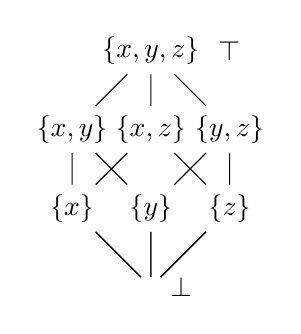
\begin{tikzpicture}[]
            \node[label={east:$\top$}] (t) at (1,4) {$\{x,y,z\}$};
            \node (xy) at (0, 3) {$\{x,y\}$};
            \node (xz) at (1, 3) {$\{x,z\}$};
            \node (yz) at (2, 3) {$\{y,z\}$};
            \node (x)  at (0, 2) {$\{x\}$};
            \node (y)  at (1, 2) {$\{y\}$};
            \node (z)  at (2, 2) {$\{z\}$};
            \node[label={east:$\bot$}] (b)  at (1, 1) {$\varnothing$};
            \draw (t) -- (xy) -- (x) -- (b) -- (y) -- (xy);
            \draw (t) -- (xz) -- (x) -- (b) -- (z) -- (xz);
            \draw (t) -- (yz) -- (y) -- (b) -- (z) -- (yz);
        \end{tikzpicture}
    \end{center}
    \caption{Poset dell'insieme delle parti $\wp(\{ x,y,z \})$}
    \label{fig:posetparti}
\end{figure}